All cold cables originating from inside the cryostat connect to the outside warm electronics through PCB board feedthroughs
installed in the signal flanges that are distributed along the cryostat roof.
The TPC data rate per APA, with an overall 32:1 MUX and 80 $\sim$1~Gbps data channels per APA,
is sufficiently low that the LVDS signals can be driven over copper twin-axial transmission lines.
Additional transmission lines are available for the distribution of LVDS clock signals and I$^2$C control information,
which are transmitted at a lower bit rate.
Optical fiber is employed externally from the WIBs on the signal flange to the DAQ and slow control systems described in Chapter~\ref{ch:fdsp-daq} and Chapter~\ref{ch:fdsp-slow-cryo}, respectively.

\begin{dunefigure}
[TPC CE feedthrough. The WIBs are seen edge-on in the left panel, and in an oblique side-view in the right panel, which also shows the warm crate for a DUNE module in a cutaway view.]
{fig:tpcelec-signal_FT}
{TPC CE feedthrough. The WIBs are seen edge-on in the left panel, and in an oblique side-view in the right panel, which also shows the warm crate for a DUNE module in a cutaway view.}
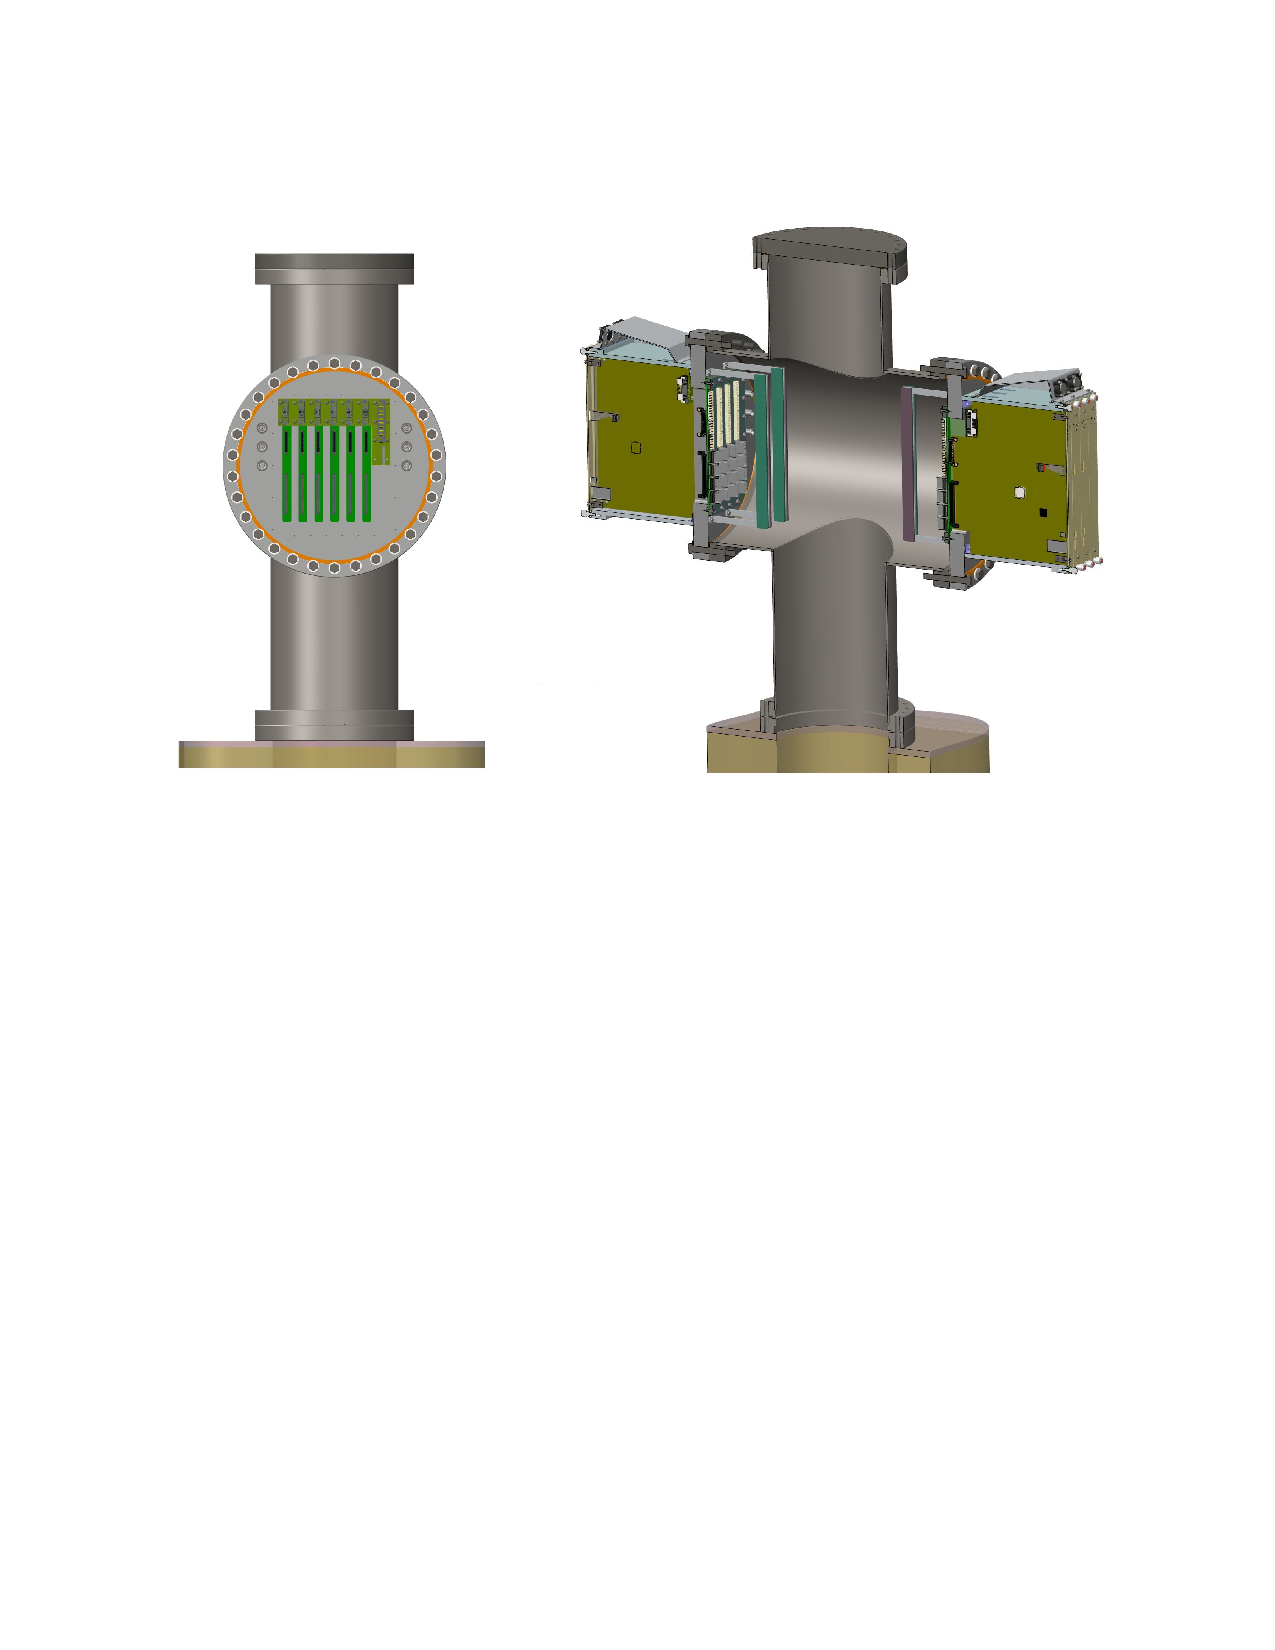
\includegraphics[width=0.9\linewidth]{tpcelec-signal_FT.pdf}
\end{dunefigure}

The design of the signal flange includes a four-way cross spool piece, separate PCB feedthroughs for the CE and PDS cables, and
an attached crate for the TPC warm electronics, as shown in Figure~\ref{fig:tpcelec-signal_FT}.
The wire bias voltage cables connect to standard SHV (safe high voltage) connectors machined directly into the CE feedthrough,
ensuring no electrical connection between the wire bias voltages and other signals passing through the signal flange.
Each CE feedthrough serves the bias/power/digital I/O needs of one APA.  

Data/control cable bundles are used to send system clock and control signals from the 
signal flange to the FEMB, stream the $\sim$1~Gbps high-speed data from the FEMB to the signal flange.  Each FEMB 
connects to a signal flange via one data cable bundle, leading to 20 bundles between one APA and one flange.  Each data bundle contains 12 low-skew twin-axial cables with a drain wire, 
to transmit the following differential signals:

\begin{itemize}
    \item four 1.28~Gbps data (two from each COLDATA);
    \item two 64~MHz clocks (one input to each COLDATA);
    \item two fast command lines (one input to each COLDATA);
    \item three I$^2$C-like control lines (clock, data-in, and data-out); and
    \item one multipurpose LArASIC output (temperature, reference voltage, or analog test output).
\end{itemize}

LV power is passed from the signal flange to the FEMB by bundles of
20AWG twisted-pair wires. Half of the wires are power feeds; the other wires
are attached to the grounds of the input amplifier circuits, as described in Section~\ref{sec:fdsp-tpc-elec-design-bias}.
For a single FEMB, the resistance is measured to be $<30$~m$\Omega$ at RT or $<10$~m$\Omega$ at 
LAr temperature. Each APA has a copper cross-section of approximately $80~\mathrm{mm}^2$, with a 
resistance $<1.5$~m$\Omega$ at RT or $<0.5$~m$\Omega$ at LAr temperature.

The bias voltages are applied to the X-, U-, and G-plane wire layers, three field cage terminations, 
and an electron diverter, as shown in Figure~\ref{fig:CR-board}. The voltages are supplied 
through eight SHV connectors mounted on the signal flange. RG-316 coaxial cables carry the voltages 
from the signal flange to a patch panel PCB which includes noise filtering mounted on the top 
end of the APA. 

From there, wire bias voltages are carried by single wires to 
various points on the APA frame, including the CR boards, a small PCB mounted on or near 
the patch panel that houses a noise filter and termination circuits for the field cage voltages, and 
a small mounted board near the electron diverter that also houses wire bias voltage filters.
